% \documentclass[a4paper]{article}
% \usepackage[ngerman]{babel}
% \usepackage[utf8]{inputenc}
% \usepackage[top=2.5cm,bottom=1.75cm,right=2cm,left=2.3cm]{geometry}
% \usepackage{wrapfig}
% \usepackage{floatflt}
% \usepackage{graphicx}
% \usepackage[colorlinks=true,linkcolor=black,bookmarksnumbered=true,breaklinks=true,pdfstartview=FitH]{hyperref}
% 
% \title{\textbf{Praktikum 10} \\ ~ \\Ultraschall II}
% 
% \author{Michael Kopp}
% 
% \date{25. Oktober 2007}
% 
% %2007-11-04 12:30
% 
% \begin{document}
% 
% 
% \maketitle


			\section{Interferenz zweier Ultraschallwellen}

		\subsection{Versuch}
\label{kap_interferenz_versuch}

\begin{figure}
   \centering
   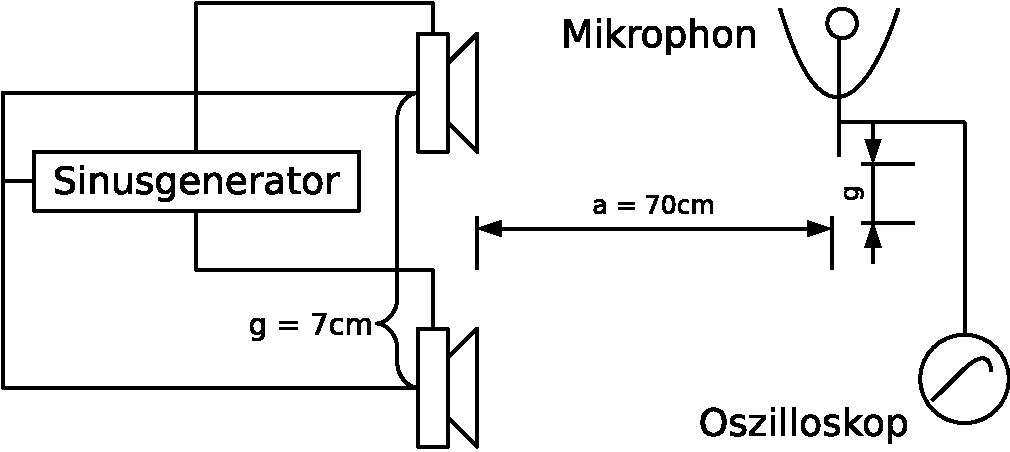
\includegraphics[width=0.8\textwidth]{praktika/mat_praktika/interferenz}
   \caption{Versuchsaufbau zum Interferenzversuch}
   \label{img_aufbau_interferenz}
\end{figure}


Zwei baugleiche Lautsprecher werden im Abstand \(g = 10cm\) voneinander parallel zueinander aufgestellt. Sie werden vom selben Sinusgenerator angesteuert und senden somit gleichphasige Schallwellen der gleichen Frequenz und Amplitude aus. Im Abstand \(a = 70cm\) senkrecht zur gedachten Verbindung der beiden Lautsprecher wird ein Mikrophon parallel zu der gedachten Verbindung um den Betrag \(g\) seitlich bewegt. Das Mikrophon ist druckempfindlich und auf einem Oszilloskop wird ausgegeben, welchen Druck es erfährt. (\(\rightarrow\) Abb. \ref{img_aufbau_interferenz}, S. \pageref{img_aufbau_interferenz})


Um die Wellenlänge des Ultraschalls zu ermitteln, stellt man das Mikrophon kurz vor einen der beiden Lautsprecher (der andere wird abgeschaltet) und verändert so lange die Frequenz am Sinusgenerator, bis die Amplitude auf dem Oszilloskop maximal wird. Auf dem Oszilloskop liest man die Periodendauer \(T = 24,4 \mu s\) ab. Somit beträgt die Frequenz \(f = \frac{1}{T} = 41kHz\). Über den Zusammenhang 
\begin{equation}
   c = \frac{\lambda}{T} = \lambda \cdot f
   \label{eq_c=lf}
\end{equation}
ergibt sich da \(c = 340 \frac{m}{s}\) eine Wellenlänge von \(\lambda \approx 8,30mm\).





		\subsection{Beobachtung}

Bewegt man das Mikrophon, so ergeben sich abwechselnd Minima und Maxima auf dem Oszilloskop. Maxima sind anzutreffen bei
\[d_{max} = \left \{ 0cm; 5,5cm; 11,5cm; 17,5cm \right \}\]
und Minima sind anzutreffen bei
\[d_{min} = \left \{ 3cm; 9cm; 15cm \right \}\]

Vertauscht man die Anschlüsse an einem der beiden Lautsprecher, so erhält man dort, wo vorher Maxima waren nun Minima und andersherum entsprechend.




		\subsection{Auswertung}

Siehe auch vorhergehendes Praktikum -- viele Rechnungen werden dort ausführlich erklärt und hier nur noch angewendet...


\subsubsection{Wellenlänge}
\label{kap_interferenz_auswertung_wellenlaenge}

Da \(a \gg g\) ist, darf man in diesem Fall die erste \textsc{Fraunhofer}-Näherung anwenden (siehe dazu Praktikum 9). Die zweite \textsc{Fraunhofer}-Näherung darf man jedoch nicht mehr anwenden, sich für große Abstände \(d\) Winkel über \(5^o\) ergeben:
\[
   \alpha = atan \left ( \frac{d}{a} \right ) = atan \left ( \frac{17,5}{70} \right ) \approx 14^o
\]
Man muss also für jeden Abstand \(d_k\) den Zugehörigen Winkel \(\alpha_k\) ausrechnen
\begin{equation}
   \alpha_k = atan \left ( \frac{d}{a} \right )
   \label{eq_alpha_k}
\end{equation}
und diesen dann in die Formel für den Gangunterschied \(\delta\) einsetzen
\begin{equation}
   \delta = g \cdot sin ( \alpha_k )
   \label{eq_delta_k}
\end{equation}
Über die Bedingungen für ein Maximum am betreffenden Punkt
\begin{equation}
   \delta = k \cdot \lambda ~~ k = (0; 1; 2; ...)
   \label{eq_bed_max}
\end{equation}
bzw. für ein Minimum
\begin{equation}
   \delta = k \cdot \lambda + \frac{\lambda}{2}~~ k = (0; 1; 2; ...)
   \label{eq_bed_min}
\end{equation}
kann man die Formeln zusammenfassen, indem man Formel \ref{eq_alpha_k} in Formel \ref{eq_delta_k} einsetzt, diese mit Formel \ref{eq_bed_max} bzw. Formel \ref{eq_bed_min} gleichsetzt und nach \(\lambda\) auflöst.

Für uns ergibt sich so für Maxima:
\begin{equation}
   \lambda_{k, max} = \frac{g \cdot sin \left ( atan \left ( \frac{d}{a} \right ) \right )}{k}
\end{equation}
und für Minima
\begin{equation}
   \lambda_{k, min} = \frac{g \cdot sin \left ( atan \left ( \frac{d}{a} \right ) \right )}{k + 0,5}
\end{equation}
Die Werte die sich nach der \textsc{Fraunhofer}-Näherung ergeben, werden in Tabelle \ref{tab_lambda_d_min} auf S. \pageref{tab_lambda_d_min} aufgeführt (für die Minima) und in Tabelle \ref{tab_lambda_d_max} auf S. \pageref{tab_lambda_d_max} (für die Maxima). 

Es ergibt sich eine schreckliche Abweichungen von \(71,68\%\). Erstaunlicherweise liegen jedoch die anderen Werte sehr nahe beieinander. Das lässt schließen, dass die allererste Messung (in Tabelle \ref{tab_lambda_d_min}) ein Ausrutscher ist. Schließlich wird die Wellenlänge bei diesem Verfahren \emph{ohne} den Ausrutscher im Mittel mit \(\lambda = 8,2mm\) berechnet (also eine Abweichung von \(-1,2\%\)) bei einer Varianz von lediglich \(V(\lambda) = 0,07mm^2\).

\begin{table}
\centering
\begin{tabular}{l|l|l|l|l|l}
\(k\)	&~~~	\(d\) [cm]	&~~~	\(\alpha\) [\(^o\)]	&~~~	\(\delta\) [cm]	&~~~	\(\lambda\) [cm]	&~~~	prozentuale Abweichung\\
\hline
0	&~~~	5	&~~~	4,09	&~~~	0,71	&~~~	1,42	&~~~	71,68\\
1	&~~~	9	&~~~	7,33	&~~~	1,28	&~~~	0,85	&~~~	2,43\\
2	&~~~	15	&~~~	12,09	&~~~	2,1	&~~~	0,84	&~~~	0,98
\end{tabular}
\caption{Berechnung der Wellenlänge aus den Werten für Minima}
\label{tab_lambda_d_min}
\end{table}


\begin{table}
\centering
\begin{tabular}{l|l|l|l|l|l}
\(k\)	&~~~	\(d\) [cm]	&~~~	\(\alpha\) [\(^o\)]	&~~~	\(\delta\) [cm]	&~~~	\(\lambda\) [cm]	&~~~	prozentuale Abweichung\\
\hline
0	&~~~	0	&~~~	0	&~~~	0	&~~~		&~~~	0\\
1	&~~~	5,5	&~~~	4,49	&~~~	0,78	&~~~	0,78	&~~~	-5,63\\
2	&~~~	11,5	&~~~	9,33	&~~~	1,62	&~~~	0,81	&~~~	-2,34\\
3	&~~~	17,5	&~~~	14,04	&~~~	2,43	&~~~	0,81	&~~~	-2,6
\end{tabular}
\caption{Berechnung der Wellenlänge aus den Werten für Maxima}
\label{tab_lambda_d_max}
\end{table}




\subsubsection{Vertauschung der Anschlüsse}


Als die beiden Anschlüsse vertauscht wurden kehrten sich Minima und Maxima um, weil die Sender nicht mehr in Phase schwangen (\(\Delta \varphi = 0\)), sondern genau gegenphasig (\(\Delta \varphi = \pi\)); schließlich wurde durch die umgedrehte Polung der Stromfluss in der Spule des Lautsprechers genau in die Gegenrichtung (bezogen sowohl auf den früheren Zustand als auch auf den anderen Lausprecher) erwirkt. Wo bei ehemaliger Polung also ein Magnetfeld so aufgebaut wurde, dass die Membran angezogen wurde wurde nun ein genau gegenläufiges Magnetfeld aufgebaut, welches die Membran abstieß und somit einen Überdruck anstatt eines Unterdrucks erzeugte.



Die Schallwelle eines der beiden Lautsprecher musste somit also die Strecke \(\frac{\lambda}{2}\) zusätzlich zurücklegen bis sie in Phase mit der gerade am anderen Lautsprecher ausgehenden Welle war.
 Die Wellen hatten also direkt bei der Erzeugung eine Phasendifferenz von \(\Delta \varphi = \pi\) und damit auf der Geraden mit stets dem selben Abstand zu beiden Lautsprechern (``MiSe'') stets einen Gangunterschied von \(\delta = \frac{\lambda}{2}\). 
Auf dieser Gerade lag somit stets ein Minimum. 
 Da zwischen einem registrierten Minimum und einem Maximum die Phasendifferenz sich stets verändert - und zwar von \(\Delta \varphi = \pi\) bis \(\Delta \varphi = 0\); also um genau \(\pi\) - hatten logischerweise die Punkte an denen vorher ein Minimum lag nun ein Maximum, weil die Phasendifferenz zwischen der MiSe und dem Vorherigen Minimum sich um \(\pi\) änderte; jetzt ebenso, und damit bei gegenphasig schwingenden Lautsprechern die Phasendifferenz auf (ein ganzzahliges Vielfaches von) \(2 \cdot \pi\) erhöht wurde, woraus wiederum ein Gangunterschied von \(\delta = 0\) resultierte, der für das Entstehen eines Maximums verantwortlich ist.  :-)
 
 
 
 



			\section{Radarfalleneffekt}

Eine Radarfalle misst auf diese Art die Geschwindigkeit von Verkehrsteilnehmern

		\subsection{Versuch}



\begin{figure}
   \centering
   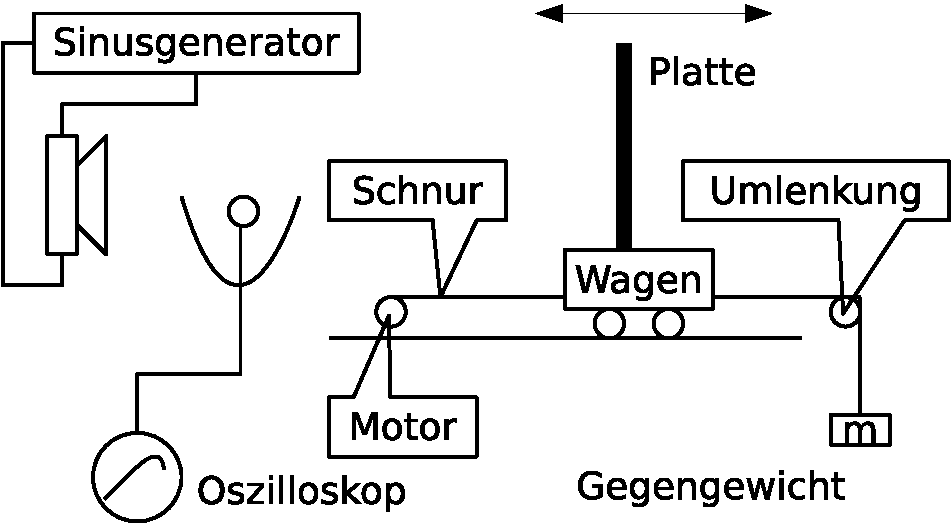
\includegraphics[width=0.8\textwidth]{praktika/mat_praktika/radar}
   \caption{Versuchsaufbau zum Versuch zum Radarfalleneffekt}
   \label{img_aufbau_radar}
\end{figure}



Auf einem Wagen, der mit der Geschwindigkeit \(v_0\) von einem Elektromotor bewegt wird, der mit einer konstanten Spannung von \(U = 0,4 V\) betrieben wird, ist eine Platte senkrecht zur Fahrtrichtung montiert. Hinter dem Wagen wird ein Lautsprecher aufgestellt und vor dem Lautsprecher ein Mikrophon, das an ein Oszilloskop gekoppelt ist.
Mit dem Oszilloskop wird gemessen, wie oft (\(n\)) in einer bestimmten Zeit \(t_0\) ein Druckbauch registriert wird.
(\(\rightarrow\) Abb. \ref{img_aufbau_radar}, S. \pageref{img_aufbau_radar})


Wie in Kapitel \ref{kap_interferenz_versuch} auf S. \pageref{kap_interferenz_versuch} muss zuerst wieder die Wellenlänge bestimmt werden. In diesem Falle ergibt sich eine Periodendauer von \(T = 8,75 \mu s\) und somit nach Formel \ref{eq_c=lf} die Wellenlänge \(\lambda = 5,95mm\).




		\subsection{Beobachtung}

Das Mikrophon registriert abwechselnd Druckminima und -maxima. In Tabelle \ref{tab_radarfalle_messwerte} auf S. \pageref{tab_radarfalle_messwerte} sind die Messwerte der verschiedenen Durchläufe festgehalten.


\begin{table}
\centering
   \begin{tabular}{c|c|c|c}
   	~~ \(t\) [sek] ~~ & ~~ \(n\) ~~ & ~~ \(v\) [\(\frac{mm}{s}\)] ~~ & ~~ prozentuale Abweichung ~~\\
   	\hline
   	37 & 68 & 5,47 & 4,3 \\
   	17 & 30 & 5,25 & -2,8 \\
   \end{tabular}
   \caption{Messwerte zum Versuch des Radarfalleneffekts}
   \label{tab_radarfalle_messwerte}

\end{table}





		\subsection{Auswertung}

Während sich der Wagen bewegt, ergibt sich ständig eine stehende Welle aus der zum Wagen hinlaufenden Welle und der vom Wagen reflektierten Welle. Dabei wird der Schalldruck an der Platte des Wagens stets ohne Phasensprung reflektiert und somit bildet sich an der Platte des Wagens stets ein Druckbauch. Von Druckbauch zu Druckbauch liegt der Abstand \(\frac{\lambda}{2}\). Zwischen den Druckbäuchen liegen Druckknoten, ebenfalls im Abstand \(\frac{\lambda}{2}\).

Misst man mit dem Oszilloskop in der Zeit \(t_0\) also \(n\) Druckknoten, so hat sich der Wagen dabei um \(s_0 = n \cdot \frac{\lambda}{2}\) bewegt, woraus sich die Geschwindigkeit 
\begin{equation}
   v_0 = \frac{s_0}{t_0} = \frac{n \cdot \frac{\lambda}{2}}{t_0} ~~~ [v_0] = \frac{mm}{s}
\end{equation}
errechnen lässt. Führt man diese Rechnung für unsere Messwerte durch, so erhält man die Ergebnisse, wie sie in Tabelle \ref{tab_radarfalle_messwerte} auf S. \pageref{tab_radarfalle_messwerte} aufgeführt sind.

festgehalten sind. Zur Kontrolle wurde die Geschwindigkeit ebenfalls bestimmt, indem die Zeit \(t_1\) gemessen wurde, die das Fahrzeug braucht, um de Strecke \(s_1 = 20cm\) zu überwinden. Demnach ist 
\[
   v_1 = \frac{s_1}{t_1} = \frac{20cm}{37sek} \approx 5,4 \frac{mm}{s}
\]
Die Abweichung unserer Werte ist ebenfalls in der Tabelle zu finden. Als Durchschnittswert für die aus unseren Messwerten berechnete Geschwindigkeit ergibt sich \(v_{0,durchschnitt} = 5,35 \frac{mm}{s}\), was mit einer Abweichung von \(-0,9\%\) als sehr präziese angesehen werden kann. 

Mögliche Ursachen für die Abweichung könnten sein:
 \begin{description}
    \item[verzählen bei Minima] Es ist bei dem Versuchsaufbau sehr einfach, dass man sich bei den Minima verzählt, weil sie so schnell auftraten und wieder verschwanden. 
    \item[Zeit stoppen] Außerdem musste man die Zeit, die der Wagen für die durchfahrenen \(20cm\) von Hand möglichst genau stoppen bzw. für das Durchlaufen der Minima, wobei ja immer reaktionsbedingte und augenmaßbedingte\footnote{Man konnte das Maßband nicht direkt an das Fahrzeug anlegen} Fehler einschleichen. 
    \item[Unregelmäßige Fahrt] Außerdem ist nicht auszuschließen, dass der Wagen nicht ganz regelmäßig auf der Schiene fuhr bzw. das Seil, welches sein Gegengewicht hielt nicht ganz regelmäßig durch die Halterung rutschte.
 \end{description}









			\section{Beugung am Gitter}



		\subsection{Versuch}


\begin{figure}
   \centering
   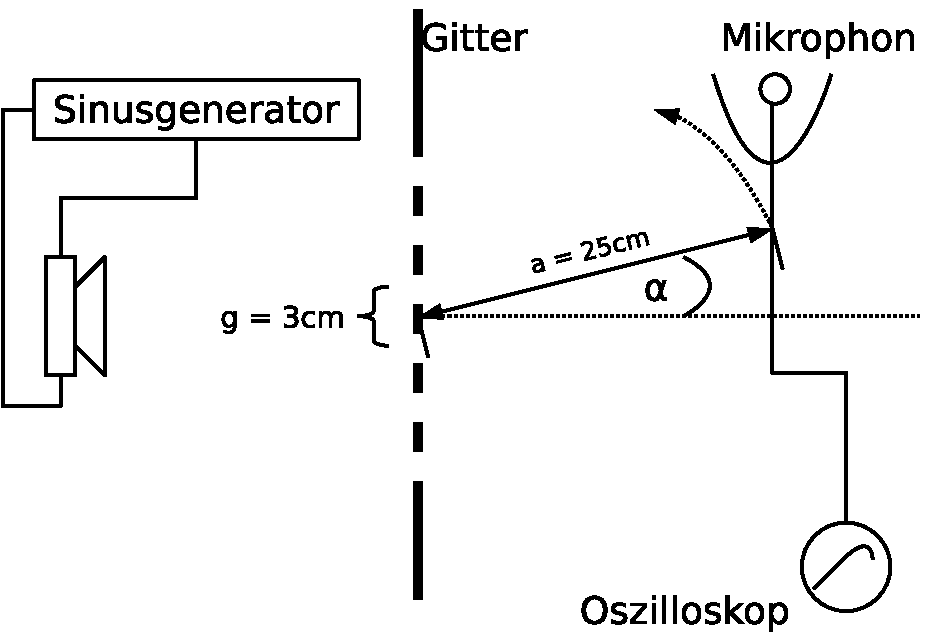
\includegraphics[width=0.8\textwidth]{praktika/mat_praktika/gitter}
   \caption{Versuchsaufbau zu Beugung am Gitter}
   \label{img_aufbau_gitter}
\end{figure}



Hinter einem Gitter mit der Gitterkonstanten \(g = 3cm\) wird ein Lautsprecher, der von einem Sinusgenerator betrieben wird, aufgestellt. In einem festen Abstand \(a = 25cm\) vom Gittermittelpunkt wird hinter dem Gitter ein Mikrophon halbkreisförmig bewegt. Das Mikrophon ist an ein Oszilloskop angeschlossen. Es registriert die Druckveränderungen. Erkennt man auf dem Oszilloskop ein Druckmaximum, so misst man den Winkel, den das Mikrophon von einer gedachten Senkrechten zum Gitter durch den Gittermittelpunkt überstrichen hat.
(\(\rightarrow\) Abb. \ref{img_aufbau_gitter}, S. \pageref{img_aufbau_gitter})

Beim bestimmen der Wellenlänge ergab sich eine Periodendauer von \(T = 21 \mu s\) und damit eine Wellenlänge von \(\lambda = 7,14mm\).



		\subsection{Beobachtungen}

In unserem Versuch ergaben sich Druckmaxima für 
\[
   \alpha_k = \left \{ 0^o; 12^o; 28^o; 58^o \right \}
\]




		\subsection{Auswertung}


Auch in diesem Falle darf man die erste \textsc{Fraunhofer}-Näherung anwenden (siehe Kap. \ref{kap_interferenz_auswertung_wellenlaenge} auf S. \pageref{kap_interferenz_auswertung_wellenlaenge}), da \(a \gg g\) gilt. Somit kann man die Wellenlänge berechnen, indem man Formel \ref{eq_delta_k} mit Formel \ref{eq_bed_max} gleichsetzt und nach \(\lambda\) auflöst:
\begin{equation}
   \lambda_k = \frac{g \cdot sin( \alpha_k )}{k}
\end{equation}
In Tabelle \ref{tab_gitter} auf S. \pageref{tab_gitter} sind die Ergebnisse der Rechnung mit der jeweiligen Abweichung von der Realität aufgeführt. Durchschnittlich ergibt sich bei unserer Messung eine Wellenlänge von \(\lambda_{durchschnitt} = 7,25mm\) bei einer Varianz von \(V(\lambda) = 1,29mm^2\) und so mit einer Standardabweichung von \(\sigma = 1,14mm\).

Gründe für die Abweichung können sein (vgl. und siehe Praktikum 9):
\begin{description}
   \item[Winkelmessen] Die Winkel mussten mit einem zu kurzen Geodreieck gemessen oder besser abgeschätzt werden
   \item[Punkte ausmachen] Es war nicht ohne weiteres möglich, die Punkte, zwischen denen die Winkel zu messen waren, auszumachen, weil dort, wo sie theoretisch sein müssten, das Stativmaterial war
   \item[Frequenz bestimmen] Die Frequenz bzw. Periodendauer zu bestimmen war nicht ganz einfach; es mussten wieder Striche auf dem Oszilloskop gezählt werden, aber manchmal war der Strahl auf dem Oszilloskop breiter aber auch so ließ sich die Periodendauer nicht besonders präzise ablesen, weil die Skala (die Markierungen auf dem Oszilloskop) zu groß gewählt war.
   \item[Maximum bestimmen] Es war nicht ganz einfach, eindeutig zu sagen, wann genau man das Maximum erreicht bzw. schon über- oder noch unterschritten hatte.
 \end{description}



\begin{table}
\centering
\begin{tabular}{l|l|l|l}
\(k\)	&~~~	\(\alpha\) [\(^o\)]	&~~~	\(\lambda\) [mm]	&~~~	prozentuale Abweichung\\
\hline
0	&~~~	0	&~~~	~	&~~~	0\\
1	&~~~	12	&~~~	6,24	&~~~	-12,64\\
2	&~~~	28	&~~~	7,04	&~~~	-1,37\\
3	&~~~	58	&~~~	8,48	&~~~	18,77
\end{tabular}
\caption{Berechnungen für die Wellenlänge bei Beugung am Gitter}
\label{tab_gitter}
\end{table}
















% \begin{appendix}
% 
% 				\section{Hinweise}
% 
% 		\subsection{Problem}
%    Unser Problem bei diesem Praktikum war, dass schlicht und ergreifend \emph{nichts} (keines der Experimente) in unserer Gruppe funktioniert hat; das Mikrophon hat von den beiden Lautsprechern unterschiedliche Frequenzen aufgezeichnet und hat man beide Lautsprecher gleichzeitig arbeiten lassen, ist das Signal völlig zusammengebrochen, betrieben wir nur ein Mikrophon, so durfte man den Abstand des Mikrophons nicht weiter verändern.
%    
%    	\subsection{Berechnung}
%    Um die Abweichungen zu berechnen wurde folgende Formel verwendet: 
% \begin{equation}
% 100 \cdot \frac{w_g - w_l}{w_l}
% \end{equation}
% Dabei ist \(w_g\) der gemessene Wert und \(w_l\) der errechnete bzw. Literaturwert.
% \end{appendix}








% 
% \end{document}
